\documentclass{article}

\usepackage{tikz}
%\usetikzlibrary{arrows}
\usepackage{marvosym}
\usepackage{graphicx}


\begin{document}

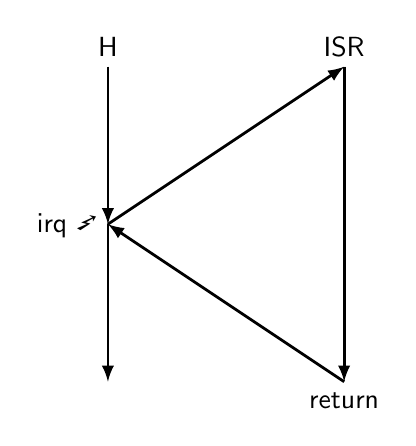
\begin{tikzpicture}[line width=1pt,font=\sffamily,-latex]
\draw (0,0)  node (H) [above] {H}  -- (0,-2) node (irq) [left] {irq \rotatebox[origin=c]{150}{\Lightning}};
\draw (0,-2) -- (3,0) node[above] {ISR};
\draw (3,0)  -- (3,-4) node[below] {return};
\draw (3,-4) -- (0,-2);
\draw (0,-2) -- (0,-4);
\end{tikzpicture}

\vspace*{1cm}

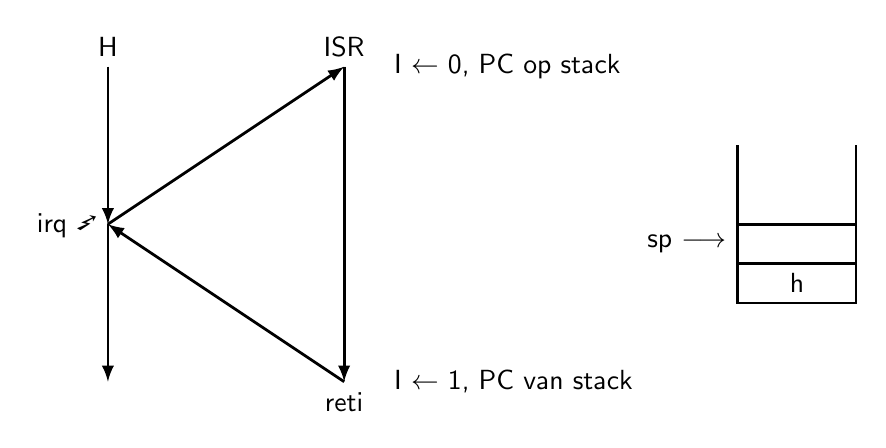
\begin{tikzpicture}[line width=1pt,font=\sffamily,-latex]
\draw (0,0)  node (H) [above] {H}  -- (0,-2) node (irq) [left] {irq \rotatebox[origin=c]{150}{\Lightning}};
\draw (0,-2) -- (3,0) node[above] {ISR} node [right, xshift=.5cm] {I $\leftarrow$ 0, PC op stack};
\draw (3,0)  -- (3,-4) node[below] {reti} node [right, xshift=.5cm] {I $\leftarrow$ 1, PC van stack};
\draw (3,-4) -- (0,-2);
\draw (0,-2) -- (0,-4);
\draw[-] (8,-1) -- ++(0,-1)
         rectangle node[xshift=-1.4cm] {sp $\longrightarrow$} ++(1.5,-0.5)
         rectangle ++(-1.5,-0.5) node[pos=.5] {h}
++(1.5,1) -- ++(0,1);
\end{tikzpicture}

\vspace*{1cm}

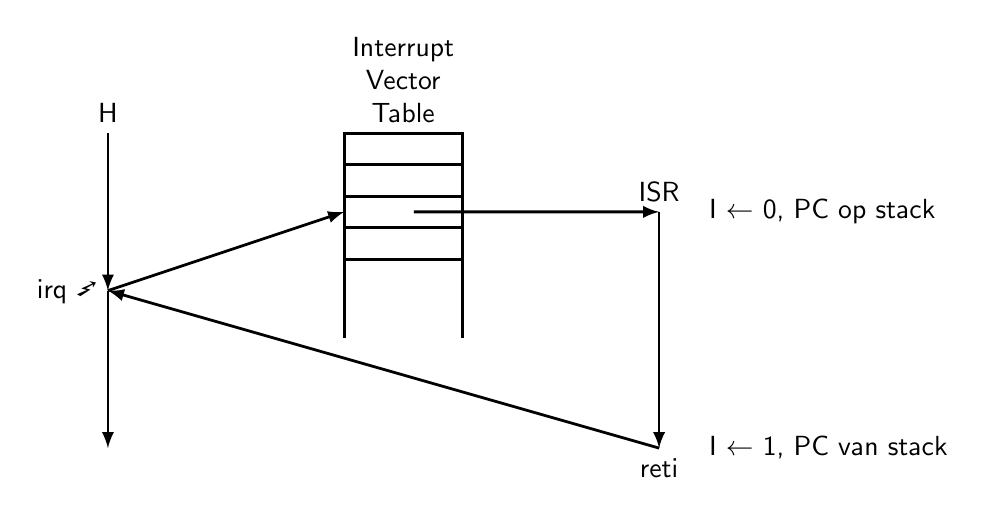
\begin{tikzpicture}[line width=1pt,font=\sffamily,-latex]
\draw (0,0)  node (H) [above] {H}  -- (0,-2) node (irq) [left] {irq \rotatebox[origin=c]{150}{\Lightning}};
\draw (3,0) rectangle ++(1.5,-0.4) node[above,pos=0.5,yshift=2mm,align=center] {Interrupt\\Vector\\Table}
            rectangle ++(-1.5,-0.4)
            rectangle ++(1.5,-0.4) node[pos=0.5] (A) {}
			rectangle ++(-1.5,-0.4)
               --     ++(0,-1)
  ++(1.5,1)    --     ++(0,-1);
\draw (0,-2) -- (3,-1);
\draw (0,-2) -- (0,-4);
\draw (A) -- (7,-1) node [above] {ISR} node [right, xshift=.5cm] {I $\leftarrow$ 0, PC op stack};
\draw (7,-1) -- (7,-4) node[below] {reti} node [right, xshift=.5cm] {I $\leftarrow$ 1, PC van stack};
\draw (7,-4) -- (0,-2);
\end{tikzpicture}


\end{document}